% ------------------------------------------------------------------------------
% TYPO3 Version 9.2 - What's New - Chapter "Changes for Integrators" (English Version)
%
% @author	Michael Schams <schams.net>
% @license	Creative Commons BY-NC-SA 3.0
% @link		http://typo3.org/download/release-notes/whats-new/
% @language	English
% ------------------------------------------------------------------------------
% LTXE-CHAPTER-UID:		3a9852ea-e2360d9d-1ff5eec1-a7de3f9f
% LTXE-CHAPTER-NAME:	Changes for Integrators
% ------------------------------------------------------------------------------

\section{Änderungen für Integratoren}
\begin{frame}[fragile]
	\frametitle{Änderungen für Integratoren}

	\begin{center}\huge{Kapitel 2:}\end{center}
	\begin{center}\huge{\color{typo3darkgrey}\textbf{Änderungen für Integratoren}}\end{center}

\end{frame}

% ------------------------------------------------------------------------------
% LTXE-SLIDE-START
% LTXE-SLIDE-UID:		7922e712-da1f1937-50e83e2d-0395df58
% LTXE-SLIDE-TITLE:		Site Handling (1)
% LTXE-SLIDE-REFERENCE:	Feature-84581-SiteHandling
% ------------------------------------------------------------------------------

\begin{frame}[fragile]
	\frametitle{Änderungen für Integratoren}
	\framesubtitle{Site Handling (1)}

	\begin{itemize}
		\item Ein neues Konzept, \textbf{Site Handling} wurde in der TYPO3 9.2 eingeführt 
		\item Backend Modul: Site Management → Configuration

	\end{itemize}

	\begin{figure}
		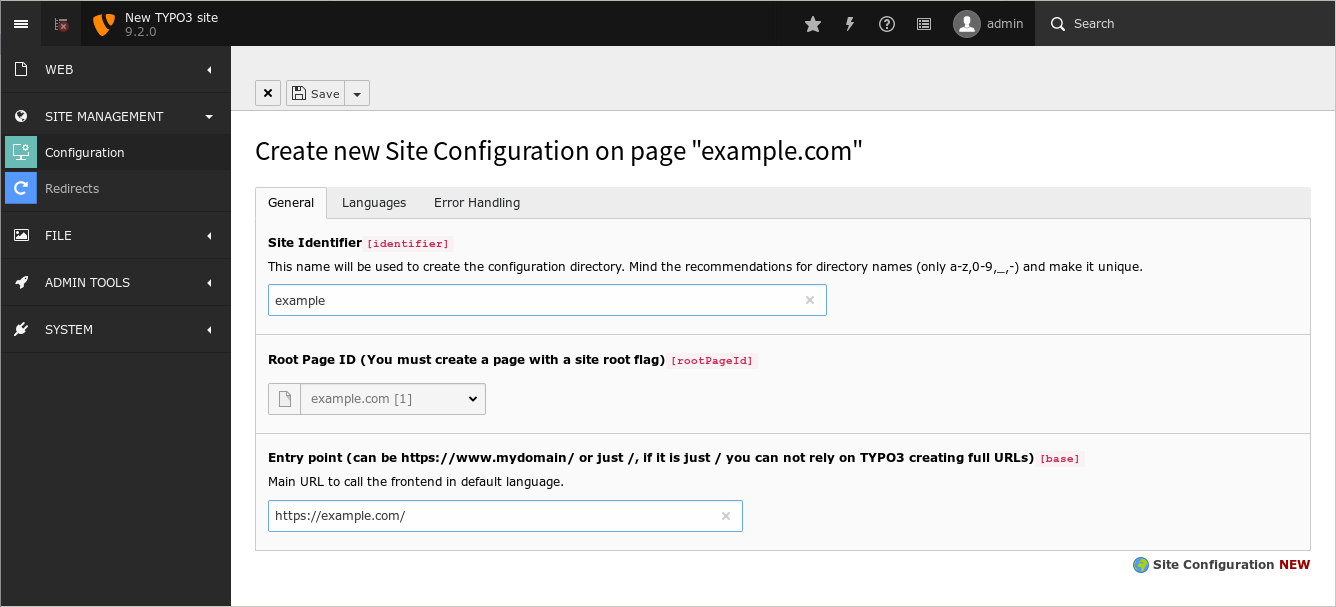
\includegraphics[width=0.85\linewidth]{ChangesForIntegrators/SiteHandling.png}
	\end{figure}

\end{frame}

% ------------------------------------------------------------------------------
% LTXE-SLIDE-START
% LTXE-SLIDE-UID:		7922e712-da1f1937-50e83e2d-0395df58
% LTXE-SLIDE-TITLE:		Site Handling (2)
% LTXE-SLIDE-REFERENCE:	Feature-84581-SiteHandling
% ------------------------------------------------------------------------------

\begin{frame}[fragile]
	\frametitle{Änderungen für Integratoren}
	\framesubtitle{Site Handling (2)}

	\begin{itemize}
		\item Die Konfigurationsdatei  enthält alle Einstellungen für eine bestimmte Seite und
			befindet sich unter \texttt{typo3conf/sites/<identifier>/config.yaml}
		\item Mögliche Bestandteile für \texttt{<identifier>}:
			\begin{itemize}
				\item \small Kleinbuchstaben/Großbuchstaben (A-Z und a-z)\normalsize
				\item \small Strich (\texttt{-})\normalsize
				\item \small Unterstrich (\texttt{\_})\normalsize
				\item \small Punkt (\texttt{.})\normalsize
			\end{itemize}
		\item Das Verzeichnis \texttt{typo3conf/sites/<identifier>/} kann in der Zukunft für zusätzliche 
			Site-bezogene Dateien verwendet werden, z.B. Fluid Templates, BE-Layouts, usw.
		\item Einige  TypoScript-Einstellungen werden basiered auf dem Inhalt von \texttt{config.yaml}
			automatisch festgelegt
	\end{itemize}

\end{frame}

% ------------------------------------------------------------------------------
% LTXE-SLIDE-START
% LTXE-SLIDE-UID:		7922e712-da1f1937-50e83e2d-0395df58
% LTXE-SLIDE-TITLE:		Mail Queue (1)
% LTXE-SLIDE-REFERENCE:	Feature-76349-IntegrateSwiftMailersSpoolTransportIntoTYPO3
% ------------------------------------------------------------------------------

\begin{frame}[fragile]
	\frametitle{Änderungen für Integratoren}
	\framesubtitle{Mail Queue (1)}

	% decrease font size for code listing
	\lstset{basicstyle=\tiny\ttfamily}

	\begin{itemize}
		\item Emails die von TYPO3 generiert sind werden sofort standardmäßig versendet
		\item TYPO3 v9.2 unterstützt 
			\href{https://example.com}{SwiftMailer's} Functionalität,
			wo die Nachricht zunächst in einer Warteschlange gespeichert wird und danach verarbeitet wird

		\item Option 1: spool Mails in dem Datenspeicher\newline
			\smaller
				(E-Mails werden nur dann versendet, wenn die Anfrage ohne Ausnahmen oder Fehler ausgeführt wurde)
			\normalsize

			\begin{lstlisting}
				$GLOBALS['TYPO3_CONF_VARS']['MAIL']['transport_spool_type'] = 'memory';
			\end{lstlisting}

		\item Option 2: spool Mails in Dateien

			\begin{lstlisting}
				$GLOBALS['TYPO3_CONF_VARS']['MAIL']['transport_spool_type'] = 'file';
				$GLOBALS['TYPO3_CONF_VARS']['MAIL']['transport_spool_filepath'] = '/folder/of/choice';
			\end{lstlisting}

	\end{itemize}

\end{frame}

% ------------------------------------------------------------------------------
% LTXE-SLIDE-START
% LTXE-SLIDE-UID:		7922e712-da1f1937-50e83e2d-0395df58
% LTXE-SLIDE-TITLE:		Mail Queue (2)
% LTXE-SLIDE-REFERENCE:	Feature-76349-IntegrateSwiftMailersSpoolTransportIntoTYPO3
% ------------------------------------------------------------------------------

\begin{frame}[fragile]
	\frametitle{Änderungen für Integratoren}
	\framesubtitle{Mail Queue (2)}

	% decrease font size for code listing
	\lstset{basicstyle=\tiny\ttfamily}

	\begin{itemize}
		\item Der folgende Konsolenbefehl kann verwendet werden, um die Queue zu verarbeiten und 
			gespoolte E-Mails zu senden.
			\newline\newline
			\small
				Alle gespoolte E-Mails verarbeiten:
			\normalsize
			\begin{lstlisting}
				$ ./typo3/sysext/core/bin/typo3 swiftmailer:spool:send
			\end{lstlisting}

			\small
				Nicht mehr als 10 gespoolte E-Mails verarbeiten:
			\normalsize
			\begin{lstlisting}
				$ ./typo3/sysext/core/bin/typo3 swiftmailer:spool:send --message-limit=10
			\end{lstlisting}

			\small
				Gespoolte E-Mails verarbeiten, aber nicht länger als 10 Sekunden:
			\normalsize
			\begin{lstlisting}
				$ ./typo3/sysext/core/bin/typo3 swiftmailer:spool:send --time-limit=10
			\end{lstlisting}

	\end{itemize}

\end{frame}

% ------------------------------------------------------------------------------
% LTXE-SLIDE-START
% LTXE-SLIDE-UID:		7922e712-da1f1937-50e83e2d-0395df58
% LTXE-SLIDE-TITLE:		AdminPanel Re-Factoring
% LTXE-SLIDE-REFERENCE:	Feature-84045-NewAdminPanelModuleAPI
% ------------------------------------------------------------------------------

\begin{frame}[fragile]
	\frametitle{Änderungen für Integratoren}
	\framesubtitle{Admin Panel Überholung}

	% change link color on this slide only
	\hypersetup{colorlinks,citecolor=blue,linkcolor=blue,menucolor=blue,filecolor=blue,anchorcolor=blue}

	\begin{itemize}

		\item Das Admin-Panel wurde erneut einer Generalüberholung unterzogen, um auf dem neuesten Stand zu sein
		\item Als erster Schritt wurde es in eine zugehörige Systemerweiterung verschoben\newline
			\smaller
				(Dadurch können Integratoren das Feature nach Bedarf aktivieren und deaktivieren)
			\normalsize

		\item Die neue API bietet flexiblere Optionen zum Hinzufügen benutzerdefinierter Module zum Admin-Panel
			oder um bestehende Module zu ersetzen\newline
			\smaller
				(siehe \hyperlink{AdminPanelCustomization}{das nächste Kapitel} für Details für Entwickler)
			\normalsize

	\end{itemize}

\end{frame}

% ------------------------------------------------------------------------------
% LTXE-SLIDE-START
% LTXE-SLIDE-UID:		7922e712-da1f1937-50e83e2d-0395df58
% LTXE-SLIDE-TITLE:		Progressive Images
% LTXE-SLIDE-REFERENCE:	Feature-48013-AddSupportForProgressiveImages
% ------------------------------------------------------------------------------

\begin{frame}[fragile]
	\frametitle{Änderungen für Integratoren}
	\framesubtitle{Progressive Bilder}

	\begin{itemize}
		\item Es ist nun möglich, progressive Bilder zu erzeugen

		\item Diese Funktion muss im Install Tool konfiguriert werden:\newline
			\small
				\texttt{\$GLOBALS['TYPO3\_CONF\_VARS']['GFX']['processor\_interlace']}
			\normalsize

		\item Mögliche Werte:
			\begin{itemize}
				\item \texttt{None}
				\item \texttt{Line}
				\item \texttt{Plane}
				\item \texttt{Partition}
			\end{itemize}

	\end{itemize}

\end{frame}

% ------------------------------------------------------------------------------
% LTXE-SLIDE-START
% LTXE-SLIDE-UID:		c7b4f7f2-a11e6fc7-4ffe6e04-92cc98aa
% LTXE-SLIDE-TITLE:		Hide Restricted Columns
% LTXE-SLIDE-REFERENCE:	Feature-83460-HideRestrictedColumns
% ------------------------------------------------------------------------------

\begin{frame}[fragile]
	\frametitle{Änderungen für Integratoren}
	\framesubtitle{Eingeschränkte Spalten}

	\begin{itemize}
		\item Spalten können im Seitenmodul ausgeblendet werden. Dadurch sehen 
			Benutzer nur die Spalten, für die Sie Inhalte bearbeiten oder hinzufügen dürfen

		\item Die folgende Einstellung in UserTS steuert das Verhalten:\newline
			\small
				\texttt{mod.web\_layout.hideRestrictedCols = 1}
			\normalsize

		\item Anmerkung: Wenn man BE-Layouts verwendet um eine abstrakte Ansicht des Front-Ends zu erhalten,
			kann das Verbergen der Spalten mit dieser Einstellung das Layout beschädigen!

	\end{itemize}

\end{frame}

% ------------------------------------------------------------------------------
% LTXE-SLIDE-START
% LTXE-SLIDE-UID:		7922e712-da1f1937-50e83e2d-0395df58
% LTXE-SLIDE-TITLE:		Environment Variable TYPO3_PATH_APP
% LTXE-SLIDE-REFERENCE:	Feature-84545-AllowTemporaryFilesToBeStoredOutsideTheDocumentRoot
% ------------------------------------------------------------------------------

\begin{frame}[fragile]
	\frametitle{Änderungen für Integratoren}
	\framesubtitle{Environment Variable \texttt{TYPO3\_PATH\_APP}}

	% decrease font size for code listing
	\lstset{basicstyle=\tiny\ttfamily}

	\begin{itemize}
		\item Die Umgebungsvariante \texttt{TYPO3\_PATH\_APP} ermöglicht das Speichern temporärer Dateien
			außerhalb des Dokuments

		\item Temporäre Dateien die sich in der Regel unter \texttt{typo3temp/var/} befinden sind
			beispielsweise Sitzungsdateien des Install Tools, Caching-Framework-Dateien, Dateien
			zum Sperren oder Protokollieren, Extension Manager-Datendateien oder Dateien,
			die von den TYPO3-Import- / Export- oder Kernaktualisierungsfunktionen generiert werden

		\item Beispielkonfiguration für den Apache-Webserver:\newline
			\smaller
				\texttt{SetEnv TYPO3\_PATH\_APP /var/www/example.com/}
			\normalsize
			\newline
			Verzeichnisaufbau:
			\newline
			\smaller
				\texttt{/var/www/example.com/htdocs/}\newline
				\texttt{/var/www/example.com/var/}
			\normalsize

	\end{itemize}

\end{frame}

% ------------------------------------------------------------------------------
% LTXE-SLIDE-START
% LTXE-SLIDE-UID:		7922e712-da1f1937-50e83e2d-0395df58
% LTXE-SLIDE-TITLE:		Miscellaneous (EXT:form Custom Validation Error Messages in Form Editor)
% LTXE-SLIDE-REFERENCE:	Feature-80124-EXTform-AllowSettingOfValidationMessagesInFormEditor.html
% LTXE-SLIDE-REFERENCE:	Feature-83506-RetrieveSessionDataInTSConditions
% ------------------------------------------------------------------------------

\begin{frame}[fragile]
	\frametitle{Änderungen für Integratoren}
	\framesubtitle{Sonstiges}

	\begin{itemize}
		\item Die neue Formularelementeigenschaft \texttt{validationErrorMessages} ermöglicht die
			Definition von benutzerdefinierten Validierungsfehlermeldungen im Formular-Editor

		\item Sessionsdaten können TypoScript-Bedingungen verwendet werden:\newline
			\small
				\texttt{[globalVar = session:foo|bar = 1234567]}
			\normalsize
			\newline
			\small
				(ehemals öffentliche Eigenschaft \texttt{sesData} is not longer available)
			\normalsize

		\item \texttt{EXT:sys\_note} Datensätze können entweder ganz oben auf der Seite oder unten auf der Seite und
			im Listenmodul gerendert werden, indem die Position im Datensatz selbst definiert wird

	\end{itemize}

\end{frame}

% ------------------------------------------------------------------------------
